\subsubsection{Voice Chat}
Sơ đồ use-case Voice chat:
\begin{figure}[H]
    \centering
    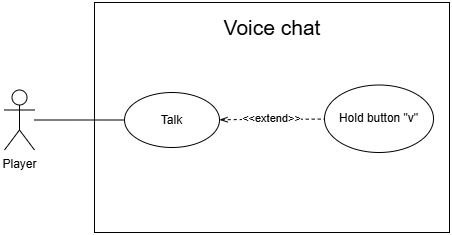
\includegraphics[width=0.75\linewidth]{4.Đặc tả chi tiết các lược đồ/Use-case/images/VoiceChat.png}
    \caption{Use-case mô tả Voice chat}
    \label{fig:placeholder}
\end{figure}


\begin{table}[H]
\centering
\begin{tabular}{|p{4cm}|p{10cm}|}
\hline
\textbf{Use-case name} & Voice chat \\ \hline
\textbf{Actor} & Người chơi \\ \hline
\textbf{Descriptions} & Use-case này sẽ chỉ ra các bước cần thực hiện để có thể sử dụng voice chat được. \\ \hline
\textbf{Pre-conditions} & Phải vào được trong lobby \\ \hline
\textbf{Trigger} & Không có. \\ \hline
\textbf{Post-conditions} & Không có \\ \hline
\textbf{Normal Flow} &
\begin{enumerate}
\item Người chơi nhấn giữ phím ''V''.
\item Người chơi bắt đầu nói chuyện bình thường.
\item Use-case kết thúc sau khi người chơi thả nút ''v''.
\end{enumerate}
\\ \hline
\textbf{Alternative Flow} &
\begin{enumerate}
\item[E1.] Tại bước 1, nếu người chơi đã bật sẵn chế độ "Push-to-talk" trong setting thì không cần bước 1 và đi đến luôn bước 2
\end{enumerate}
\\ \hline
\textbf{Exception Flow} &
Không có
\\ \hline
\end{tabular}
\end{table}